% !TeX spellcheck = sl_SI
% vim: set spell spelllang=sl:
% za preverjanje črkovanja, če se uporablja Texstudio ali vim
\documentclass[12pt,a4paper,twoside]{article}
\usepackage[utf8]{inputenc}  % pravilno razpoznavanje unicode znakov

% NASLEDNJE UKAZE USTREZNO POPRAVI
\newcommand{\program}{Matematika} % ime studijskega programa
\newcommand{\imeavtorja}{Marija Novak} % ime avtorja
\newcommand{\imementorja}{prof.~dr.~Janez Novak} % akademski naziv in ime mentorja, uporabi poln naziv, prof.~dr.~, doc.~dr., ali izr.~prof.~dr.
\newcommand{\imesomentorja}{} % akademski naziv in ime somentorja, če ga imate
\newcommand{\naslovdela}{Naslov vašega dela}
\newcommand{\letnica}{2017} % letnica magistriranja
\newcommand{\opis}{Delo obravnava integracijo po ω-kompleksih, njene lastnosti in posplošitve
na Levy-jeve topološke prostore.}  % Opis dela v eni povedi. Ne sme vsebovati matematičnih simbolov v $ $.
\newcommand{\kljucnebesede}{integracija\sep kompleks} % ključne besede, ločene z \sep, da se PDF metapodatki prav procesirajo
\newcommand{\keywords}{integration\sep complex} % ključne besede v angleščini
\newcommand{\organization}{Univerza v Ljubljani, Fakulteta za matematiko in fiziko} % fakulteta
\newcommand{\literatura}{literatura}  % pot do datoteke z literaturo (brez .bib končnice)
\newcommand{\sep}{, }  % separator med ključnimi besedami v besedilu
% KONEC PODATKOV

\usepackage{bibentry}         % za navajanje literature v programu dela s celim imenom
\nobibliography{\literatura}
\newcommand{\plancite}[1]{\item[\cite{#1}] \bibentry{#1}} % citiranje v programu dela

\usepackage{filecontents}  % za pisanje datoteke s PDF metapodatki
\usepackage{silence} \WarningFilter{latex}{Overwriting file}  % odstrani annoying warning o obstoju datoteke
% datoteka s PDF metapodatki, zgenerira se kot magisterij.xmpdata
\begin{filecontents*}{\jobname.xmpdata}
  \Title{\naslovdela}
  \Author{\imeavtorja}
  \Keywords{\kljucnebesede}
  \Subject{\opis}
  \Org{\organization}
\end{filecontents*}

\usepackage[a-1b]{pdfx}  % zgenerira PDF v tem PDF/A-1b formatu, kot zahteva knjižnica
\hypersetup{bookmarksopen, bookmarksdepth=3, colorlinks=true,
  linkcolor=black, anchorcolor=black, citecolor=black, filecolor=black,
  menucolor=black, runcolor=black, urlcolor=black, pdfencoding=auto,
  breaklinks=true, psdextra}

\usepackage[slovene]{babel}  % slovenščina
\usepackage[T1]{fontenc}     % naprednejše kodiranje fonta
\usepackage{amsmath,amssymb,amsfonts,amsthm} % matematični paketi
\usepackage[dvipsnames,usenames]{color} % barve
\usepackage{graphicx}     % za slike
\usepackage{emptypage}    % prazne strani so neoštevilčene, ampak so štete
\usepackage{units}        % fizikalne enote kot \unit[12]{kg} s polovico nedeljivega presledka, glej primer v kodi
\usepackage{makeidx}      % za stvarno kazalo, lahko zakomentiraš, če ne rabiš
\makeindex                % za stvarno kazalo, lahko zakomentiraš, če ne rabiš
% oblika strani
\usepackage[
  top=3cm,
  bottom=3cm,
  inner=3.5cm,      % margini za dvostransko tiskanje
  outer=2.5cm,
  footskip=40pt     % pozicija številke strani
]{geometry}

% VEČ ZANIMIVIH PAKETOV
% \usepackage{array}      % več možnosti za tabele
% \usepackage[list=true,listformat=simple]{subcaption}  % več kot ena slika na figure, omogoči slika 1a, slika 1b
% \usepackage[all]{xy}    % diagrami
% \usepackage{doi}        % za clickable DOI entrye v bibliografiji
% \usepackage{enumerate}     % več možnosti za sezname

% Za barvanje source kode
% \usepackage{minted}
% \renewcommand\listingscaption{Program}

% Za pisanje psevdokode
% \usepackage{algpseudocode}  % za psevdokodo
% \usepackage{algorithm}
% \floatname{algorithm}{Algoritem}
% \renewcommand{\listalgorithmname}{Kazalo algoritmov}

% DRUGI TVOJI PAKETI:
% tukaj

\setlength{\overfullrule}{50pt} % označi predlogo vrstico
\pagestyle{plain}               % samo številka strani na dnu, nobene glave / noge

% ukazi za matematična okolja
\theoremstyle{definition} % tekst napisan pokončno
\newtheorem{definicija}{Definicija}[section]
\newtheorem{primer}[definicija]{Primer}
\newtheorem{opomba}[definicija]{Opomba}
\newtheorem{aksiom}{Aksiom}

\theoremstyle{plain} % tekst napisan poševno
\newtheorem{lema}[definicija]{Lema}
\newtheorem{izrek}[definicija]{Izrek}
\newtheorem{trditev}[definicija]{Trditev}
\newtheorem{posledica}[definicija]{Posledica}

\numberwithin{equation}{section}  % števec za enačbe zgleda kot (2.7) in se resetira v vsakem poglavju

% Matematični ukazi
\newcommand{\R}{\mathbb R}
\newcommand{\N}{\mathbb N}
\newcommand{\Z}{\mathbb Z}
\renewcommand{\C}{\mathbb C}
\newcommand{\Q}{\mathbb Q}

% \DeclareMathOperator{\tr}{tr}  % morda potrebuješ operator za sled ali kaj drugega?

% bold matematika znotraj \textbf{ }, tudi v naslovih, kot \omega spodaj
\makeatletter \g@addto@macro\bfseries{\boldmath} \makeatother

% Poimenuj kazalo slik kot ``Kazalo slik'' in ne ``Slike''
\addto\captionsslovene{
  \renewcommand{\listfigurename}{Kazalo slik}%
}

% če želiš, da se poglavja začnejo na lihih straneh zgoraj
% \let\oldsection\section
% \def\section{\cleardoublepage\oldsection}

%%%%%%%%%%%%%%%%%%%%%%%%%%%%%%%%%%%%%%%%%%
%%%%%%           DOCUMENT           %%%%%%
%%%%%%%%%%%%%%%%%%%%%%%%%%%%%%%%%%%%%%%%%%

\begin{document}

\pagenumbering{roman} % začnemo z rimskimi številkami
\thispagestyle{empty} % ampak na prvi strani ni številke

\noindent{\large
UNIVERZA V LJUBLJANI\\[1mm]
FAKULTETA ZA MATEMATIKO IN FIZIKO\\[5mm]
\program\ -- 2.~stopnja}
% ustrezno dopolni za IŠRM
\vfill

\begin{center}
  \large
  \imeavtorja\\[3mm]
  \Large
  \textbf{\MakeUppercase{\naslovdela}}\\[10mm]
  \large
  Magistrsko delo \\[1cm]
  Mentor: \imementorja \\[2mm] % ustrezno popravi spol
%   Somentor: \imesomentorja   % dodaj, če potrebno
\end{center}
\vfill

\noindent{\large Ljubljana, \letnica}

\cleardoublepage

%% IZJAVA O AVTORSTVU
%\pdfbookmark[1]{Izjava o avtorstvu}{izjava} % bookmark v PDF, \pdfbookmark[nivo]{text}{label}
%
%% izjava: po potrebi spremeni v žensko obliko
%\setlength\topsep{0pt}
%\setlength\parskip{0pt}
%\begin{center}
%  \textbf{Univerza v Ljubljani} \\
%  \textbf{Fakulteta za matematiko in fiziko}
%
%  \vfill
%
%  \underline{Izjava o avtorstvu, istovetnosti tiskane in elektronske verzije magistrskega dela in} \\
%  \underline{objavi osebnih podatkov študenta}
%
%  \vfill
%
%  \setlength\topsep{0pt}
%  \setlength\parskip{0pt}
%  \begin{flushleft}
%    Spodaj podpisani študent \imeavtorja{} avtor magistrskega dela (v nadaljevanju: pisnega
%    zaključnega dela študija) z naslovom:
%  \end{flushleft}
%
%  \vfill
%
%  \textbf{\naslovdela}
%
%  \vfill
%
%  IZJAVLJAM
%\end{center}
%
%\begin{enumerate}[1. ]
%  \item \emph{Obkrožite eno od variant a) ali b)}
%  \begin{enumerate}[a)]
%    \item da sem pisno zaključno delo študija izdelal samostojno;
%    \item da je pisno zaključno delo študija rezultat lastnega dela več kandidatov in izpolnjuje
%      pogoje, ki jih Statut UL določa za skupna zaključna dela študija ter je v zahtevanem deležu
%      rezultat mojega samostojnega dela;
%  \end{enumerate}
%  pod mentorstvom IZPOLNI. % dopiši \imementorja v rodilniku
%%   \\ in somentorstvom IZPOLNI. % dopiši \imesomentorja v rodilniku
%  \item da je tiskana oblika pisnega zaključnega dela študija istovetna elektronski obliki
%    pisnega zaključnega dela študija;
%  \item da sem pridobil vsa potrebna dovoljenja za uporabo podatkov in avtorskih del v pisnem
%    zaključnem delu študija in jih v pisnem zaključnem delu študija jasno označil;
%  \item da sem pri pripravi pisnega zaključnega dela študija ravnal v skladu z etičnimi načeli in,
%    kjer je to potrebno, za raziskavo pridobil soglasje etične komisije;
%  \item da soglašam, da se elektronska oblika pisnega zaključnega dela študija uporabi za preverjanje
%    podobnosti vsebine z drugimi deli s programsko  opremo za preverjanje podobnosti
%    vsebine, ki je povezana s študijskim informacijskim sistemom fakultete;
%  \item da na UL neodplačno, neizključno, prostorsko in časovno neomejeno prenašam pravico shranitve
%    avtorskega dela v elektronski obliki, pravico reproduciranja ter pravico dajanja pisnega
%    zaključnega dela študija na voljo javnosti na svetovnem spletu preko Repozitorija UL;
%  \item da dovoljujem objavo svojih osebnih podatkov, ki so navedeni v pisnem zaključnem delu študija
%    in tej izjavi, skupaj z objavo pisnega zaključnega dela študija.
%\end{enumerate}
%
%\vfill
%
%\noindent
%Kraj:  \hfill   Podpis študenta: \phantom{prostor za podpis}
%
%\vfill
%
%\noindent
%Datum:
%
%\cleardoublepage
%% END IZJAVA O AVTORSTVU

% zahvala
\pdfbookmark[1]{Zahvala}{zahvala} %
\section*{Zahvala}
Neobvezno.
Zahvaljujem se \dots
% end zahvala -- izbriši vse med zahvala in end zahvala, če je ne rabiš

\cleardoublepage

\pdfbookmark[1]{\contentsname}{kazalo-vsebine}
\tableofcontents

% list of figures
% \cleardoublepage
% \pdfbookmark[1]{\listfigurename}{kazalo-slik}
% \listoffigures
% end list of figures

\cleardoublepage

\section*{Program dela}
\addcontentsline{toc}{section}{Program dela} % dodajmo v kazalo
Mentor naj napiše program dela skupaj z osnovno literaturo. Na literaturo se
lahko sklicuje kot~\cite{lebedev2009introduction}, \cite{gurtin1982introduction},
\cite{zienkiewicz2000finite}, \cite{STtemplate}.

\section*{Osnovna literatura}
Literatura mora biti tukaj posebej samostojno navedena (po pomembnosti) in ne
le citirana. V tem razdelku literature ne oštevilčimo po svoje, ampak uporabljamo
okolje itemize in ukaz plancite, saj je celotna literatura oštevilčena na koncu.
\begin{itemize}
  \plancite{lebedev2009introduction}
  \plancite{gurtin1982introduction}
  \plancite{zienkiewicz2000finite}
  \plancite{STtemplate}
\end{itemize}

\vspace{2cm}
\hspace*{\fill} Podpis mentorja: \phantom{prostor za podpis}

% \vspace{2cm}
% \hspace*{\fill} Podpis somentorja: \phantom{prostor za podpis}

\cleardoublepage
\pdfbookmark[1]{Povzetek}{abstract}

\begin{center}
\textbf{\naslovdela} \\[3mm]
\textsc{Povzetek} \\[2mm]
\end{center}
Tukaj napišemo povzetek vsebine. Sem sodi razlaga vsebine in ne opis tega, kako je delo
organizirano.

\vfill
\begin{center}
\textbf{English translation of the title} \\[3mm] % prevod slovenskega naslova dela
\textsc{Abstract}\\[2mm]
\end{center}

An abstract of the work is written here. This includes a short description of
the content and not the structure of your work.

\vfill\noindent
\textbf{Math.~Subj.~Class.~(2010):} oznake kot 74B05, 65N99, na voljo so na naslovu
\url{http://www.ams.org/msc/msc2010.html?t=65Mxx} \\[1mm]
\textbf{Ključne besede:} \kljucnebesede \\[1mm]
\textbf{Keywords:} \keywords

\cleardoublepage

\setcounter{page}{1}    % od sedaj naprej začni zopet z 1
\pagenumbering{arabic}  % in z arabskimi številkami

\section{Uvod}
Napišite kratek zgodovinski in matematični uvod.  Pojasnite motivacijo za problem, kje
nastopa, kje vse je bil obravnavan. Na koncu opišite tudi organizacijo dela -- kaj je v kakšnem
razdelku.

\section{Integrali po \texorpdfstring{$\omega$}{ω}-kompleksih}
\subsection{Definicija}
\begin{definicija}
  Neskončno zaporedje kompleksnih števil, označeno z $\omega = (\omega_1, \omega_2, \ldots)$,
  se imenuje \emph{$\omega$-kompleks}.\footnote{To ime je izmišljeno.}

  Črni blok zgoraj je tam namenoma. Označuje, da \LaTeX{} ni znal vrstice prelomiti pravilno
  in vas na to opozarja. Preoblikujte stavek ali mu pomagajte deliti problematično besedo z
  ukazom \verb|\hyphenation{an-ti-ko-mu-ta-ti-ven}| v preambuli.
\end{definicija}
\begin{trditev}[Znano ime ali avtor]
  \label{trd:obstoj-omega}
  Obstaja vsaj en $\omega$-kompleks.
\end{trditev}
\begin{proof}
  Naštejmo nekaj primerov:
  \begin{align}
    \omega &= (0, 0, 0, \dots), \label{eq:zero-kompleks} \\
    \omega &= (1, i, -1, -i, 1, \ldots), \nonumber \\
    \omega &= (0, 1, 2, 3, \ldots). \nonumber \qedhere  % postavi QED na zadnjo vrstico enačbe
  \end{align}
\end{proof}

\section{Tehnični napotki za pisanje}

\subsection{Sklicevanje in citiranje}
Za sklice uporabljamo \verb|\ref|, za sklice na enačbe \verb|\eqref|, za citate \verb|\cite|. Pri
sklicevanju in citiranju sklicano številko povežemo s prejšnjo besedo z nedeljivim presledkom
$\sim$, kot npr.\ \verb|iz trditve~\ref{trd:obstoj-omega} vidimo|.

\begin{primer}
  Zaporedje~\eqref{eq:zero-kompleks} iz dokaza trditve~\ref{trd:obstoj-omega} na
  strani~\pageref{trd:obstoj-omega} lahko najdemo tudi v Spletni enciklopediji zaporedij~\cite{oeis}.
  Citiramo lahko tudi bolj natančno~\cite[trditev 2.1, str.\ 23]{lebedev2009introduction}.
\end{primer}

\subsection{Okrajšave}
Pri uporabi okrajšav \LaTeX{} za piko vstavi predolg presledek, kot npr. tukaj. Zato se za vsako
piko, ki ni konec stavka doda presledek običajne širine z ukazom \verb*|\ |, kot npr.\ tukaj.
Primerjaj z okrajšavo zgoraj za razliko.

\subsection{Vstavljanje slik}
Sliko vstavimo v plavajočem okolju \texttt{figure}. Plavajoča okolja \emph{plavajo} po tekstu, in
jih lahko postavimo na vrh strani z opcijskim parametrom `\texttt{t}', na lokacijo, kjer je v kodi s
`\texttt{h}', in če to ne deluje, potem pa lahko rečete \LaTeX u, da ga \emph{res} želite tukaj,
kjer ste napisali, s `\texttt{h!}'. Lepo je da so vstavljene slike vektorske (recimo \texttt{.pdf}
ali \texttt{.eps} ali \texttt{.svg}) ali pa \texttt{.png} visoke resolucije (več kot
\unit[300]{dpi}).  Pod vsako sliko je napis in na vsako sliko se skličemo v besedilu. Primer
vektorske slike je na sliki~\ref{fig:sample}. Vektorsko sliko prepoznate tako, da močno
zoomate v sliko, in še vedno ostane gladka. Več informacij je na voljo na
\url{https://en.wikibooks.org/wiki/LaTeX/Floats,_Figures_and_Captions}. Če so slike bitne, kot na
primer slika~\ref{fig:image}, poskrbite, da so v dovolj visoki resoluciji.

\begin{figure}[h]
  \centering
  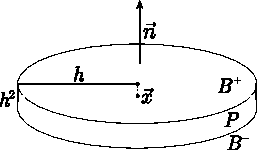
\includegraphics[width=0.6\textwidth]{images/sample.pdf}
% \caption[caption za v kazalo]{Dolg caption pod sliko}
  \caption[Primer vektorske slike.]{Primer vektorske slike z oznakami v enaki pisavi, kot jo
     uporablja \LaTeX{}.  Narejena je s programom Inkscape, \LaTeX{} oznake so importane v
     Inkscape iz pomožnega PDF.}
  \label{fig:sample}
\end{figure}

\begin{figure}[h]
  \centering
  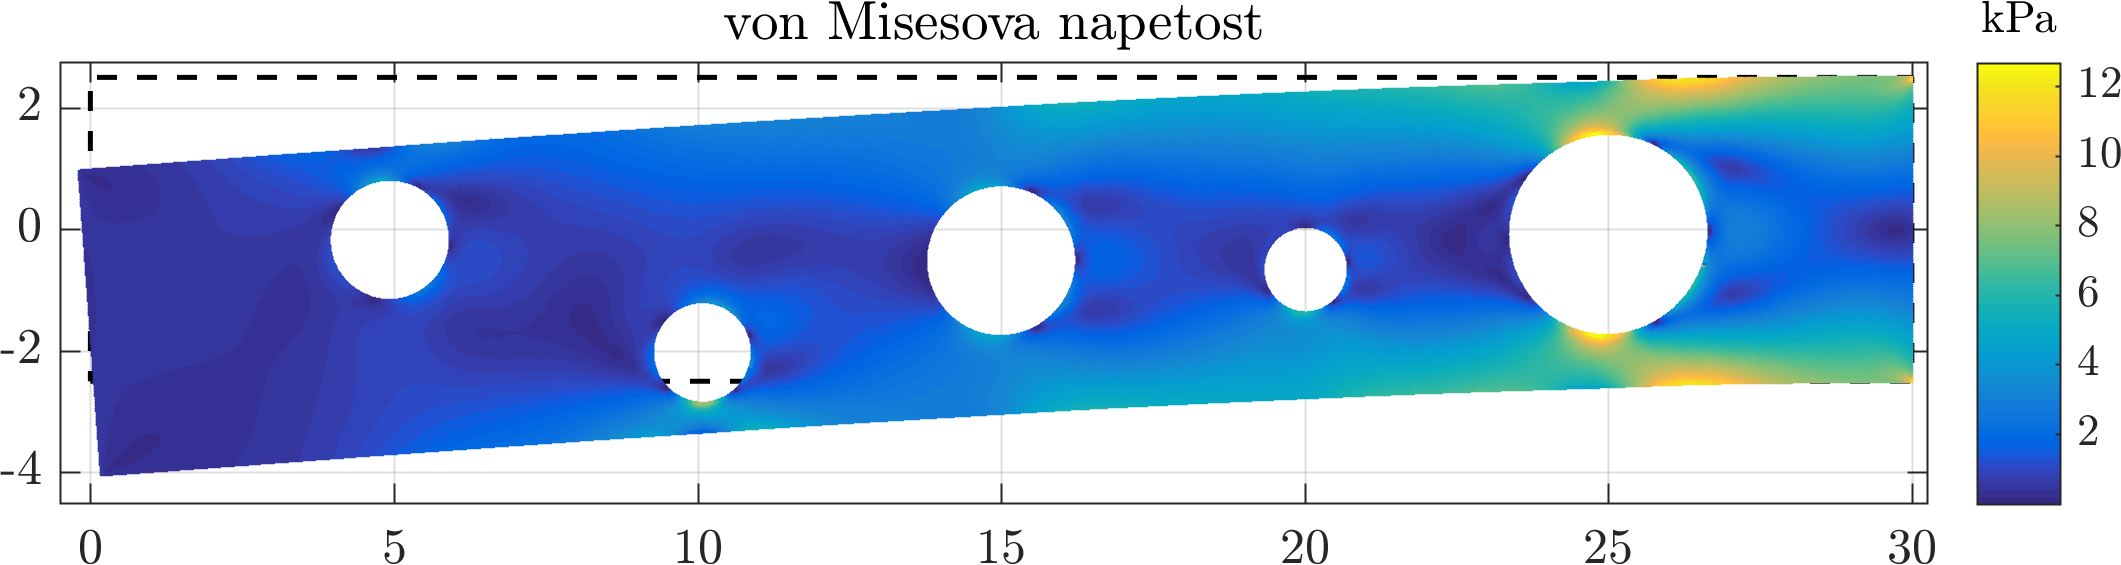
\includegraphics[width=0.8\textwidth]{images/image.png}
  \caption[Primer bitne slike.]{Primer bitne slike, izvožene iz Matlaba. Poskrbite, da so slike v
  dovolj visoki resoluciji in da ne vsebujejo prosojnih elementov (to zahteva PDF/A-1b format).}
  \label{fig:image}
\end{figure}

\subsection{Kako narediti stvarno kazalo}
Dodate ukaze \verb|\index{polje}| na besede, kjer je pojavijo, kot tukaj\index{tukaj}.
Več o stvarnih kazalih je na voljo na \url{https://en.wikibooks.org/wiki/LaTeX/Indexing}.

\subsection{Navajanje literature}
Članke citiramo z uporabo \verb|\cite{label}|, \verb|\cite[text]{label}| ali pa več naenkrat s
\verb|\cite\{label1, label2}|. Tudi tukaj predhodno besedo in citat povežemo z nedeljivim presledkom
$\sim$. Na primer~\cite{chen2006meshless,liu2001point}, ali pa \cite{kibriya2007empirical}, ali pa
\cite[str.\ 12]{trobec2015parallel}, \cite[enačba (2.3)]{pereira2016convergence}.
Vnosi iz \verb|.bib| datoteke, ki niso citirani, se ne prikažejo v seznamu literature, zato jih
tukaj citiram.~\cite{vene2000categorical}, \cite{gregoric2017stopniceni}, \cite{slak2015induktivni},
\cite{nsphere}, \cite{kearsley1975linearly}, \cite{STtemplate}, \cite{NunbergerTand}.

% Literatura:
% Primer navajanja na http://www.fmf.uni-lj.si/storage/24240/LiteraturaM.pdf,
% ampak bi moral stil poskrbeti za vse. Reference se uredijo po abecedi.
% Če nobena izbira izmed @book, @atricle,... ni ok, potem se lahko vse napiše v
% @misc pod note={} in deluje tako kot normalen LaTeX.
% Komentar v bib datoteki se naredi samo s parom { }
% Za urejanje literature avtor priporoča program Jabref, ki zna tudi avtomatsko
% okrajšati imena revij. Za pravilno sortiranje vnosov brez avtorja, uporabite
% polje key={ }, kot v primeru.
% V primeru napak ustvarite issue na GitHubu ali pišite na jure.slak@fmf.uni-lj.si.
\cleardoublepage                           % na desni strani
\phantomsection                            % da prav delujejo hiperlinki
\addcontentsline{toc}{section}{\bibname}   % dodajmo v kazalo
\bibliographystyle{fmf-sl}                 % uporabljen stil je v datoteki fmf-sl.bst, na voljo tudi angleška verzija
\bibliography{\literatura}                 % literatura je v datoteki, definirani na začetku

% Za stvarno kazalo
\cleardoublepage                           % na desni strani
\phantomsection                            % da prav delujejo hiperlinki
\addcontentsline{toc}{section}{\indexname} % dodajmo v kazalo
\printindex

\end{document}
